\documentclass[11pt,a4paper,oneside]{article}
% Essential
\usepackage[english]{babel}
\usepackage{fancyhdr}
\usepackage{titling}
% Optional
\usepackage{hyperref}
\usepackage{amsmath}
\usepackage{graphicx}
\usepackage{listings}
\usepackage{tikz}	
\usepackage{multicol}
\usepackage{float}
\usepackage{amsmath}
\usepackage{longtable} 
\usepackage[official]{eurosym}
\usepackage{xcolor}


\graphicspath{{figures/}}
\restylefloat{figure}
 
% Titlepage
\newcommand\maintitle{Genetic Algorithms (ATHENS course): Takehome project report}
\newcommand\teacherstitle{\large E. Sidiropoulos \\ C. Evangelides}
\title{\maintitle \\ \teacherstitle}
\date{\today}
\author{Dieter Castel}
 
% Margins
\setlength{\topmargin}{0in}
\setlength{\footskip}{0.5in}
\setlength{\textwidth}{6.5in}
\setlength{\oddsidemargin}{0in}
\setlength{\evensidemargin}{0in}
\setlength{\textheight}{8.5in}
 
% Header configuration
\pagestyle{fancy}
\fancyhead{} 
\fancyhead[L]{\maintitle}
\fancyhead[R]{\thedate}
\fancyfoot{}
\fancyfoot[L]{\theauthor}
\fancyfoot[R]{\thepage}
\renewcommand{\headrulewidth}{0.4pt}
\renewcommand{\footrulewidth}{0.4pt}

\lstdefinestyle{matlab}{
  belowcaptionskip=1\baselineskip,
  breaklines=true,
  frame=L,
  xleftmargin=\parindent,
  language=Matlab,
  showstringspaces=false,
  basicstyle=\footnotesize\ttfamily,
  keywordstyle=\bfseries\color{green!40!black},
  commentstyle=\itshape\color{purple!40!black},
  identifierstyle=\color{blue},
  stringstyle=\color{orange},
  numbers=left,
  numberstyle=\tiny,
  stepnumber=1,
}

\lstdefinestyle{matlab_output}{
  belowcaptionskip=1\baselineskip,
  breaklines=true,
  frame=single,
  xleftmargin=\parindent,
  showstringspaces=false,
  basicstyle=\footnotesize,
}
\begin{document}
\maketitle
\tableofcontents
%\listoffigures
%\lstlistoflistings
\newpage

\section{Introduction}
The assignment describes the problem a fire department would have if they want to select the best location for placing a fire unit.
There are 50 locations suitable and those are spaced out evenly on a grid as shown in figure \ref{fig:assig}.
The river in the center of the town has two bridges.
These bridges should be taken into account when calculating the weight each point gets according to the objective function.
The objective function models the response time to all these locations according to the distance. In the next section we will look at this function in more detail.
\begin{figure}
		\centering
		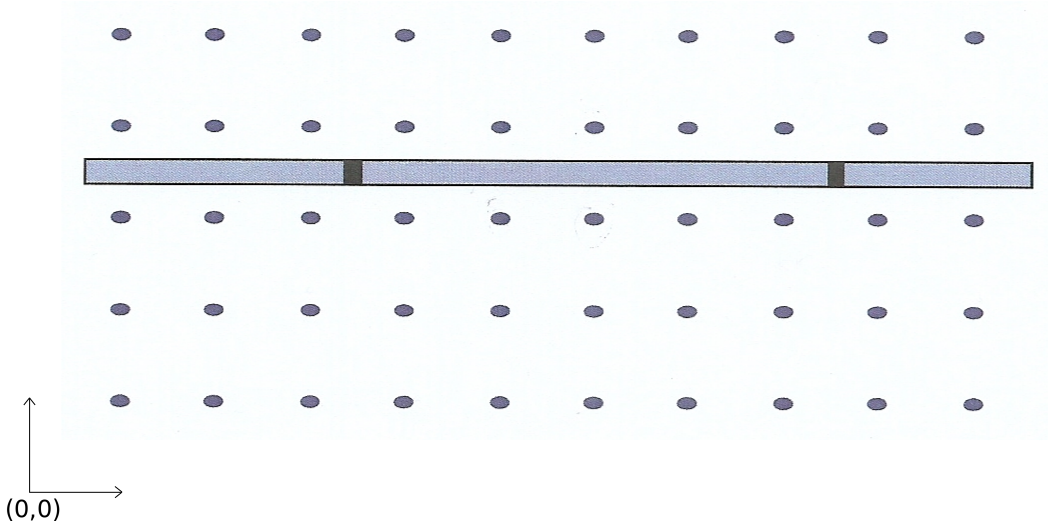
\includegraphics[scale=0.3]{assignment.png}
		\caption{Graphical representation of the town with the 50 possible locations. Each dot represents a possible building site for the fire unit. The rectangle in the center of the image is the river with the two bridges at $(3.5,3.5)$ and $(8.5,8.5)$}
		\label{fig:assig}
\end{figure}

\section{Objective function}
The objective function for this particular problem is defined as the summed distance to each of the possible building sites.
The euclidean distance is being used and the bridges are taken into account.
The euclidean distance is proffered over an other distance (e.g. hamming distance) since we have no further information about the layout of the town.
The symbolic notation of the objective function is the following:

$$f((a,b)) =  \Sigma_{x \in i, y \in j} (x - a)^2 + (y - b)^2 $$
$$\text{with } i = {1,\ldots,10}\text{ and }j ={1,\ldots,5}$$

The Matlab implementation of the objective function $f$ can be found in listing \ref{l:weight} on page \pageref{l:weight}.

In figure \ref{fig:mesh} you can find a graphical representation of the objective function $f$.
The choice to represent the function in a mesh grid is intentional. 
Because creating a mesh grid isn't as calculation intensive as a more precise representation, a rough idea can quickly be formed of the function being researched.

In this case it is clear that there seems to be a minimum in the region between 2 and 4 in both the x and y direction. With this in mind we can easily evaluate the algorithms we wrote for the problem.

\begin{figure}
		\centering
		\includegraphics{mesh.png}
		\caption{A mesh visualization of the objective function. A grid of 10 on 10 is used starting in point (0,0). Under the mesh the contour plot is visible.}
		\label{fig:mesh}
\end{figure}
\section{Search space specification}
Since only a finite amount of possible locations is given the search space is clearly discrete. The (two-dimensional) points were defined in the previous section as the combination of all the elements from $i$ for the first dimension with every element of $j$ for the second dimension.

\section{Genetic Algorithm}
For the genetic algorithm we take a two dimensional coordinate as chromosome.
Initially the population is randomly generated with each coordinate picked from a uniform distribution between 1 and 10. 
In this algorithm as much parents will survive as the amount of children they create.
The parents are selected in order of their respective weights (lowest is best for this problem).
To give more chances to reproduce to better parents an exponential distribution is used depending on the amount of parents selected.
Randomly the first or second gene is selected from one parent and combined with the other gene of another parent.
After combining the two genes on each of the genes there is a small chance of mutation (either positive or negative unit).
This new combinations gives us the children which form, in addition to the parents and survivors, the new generation. 
\subsection{code}
\lstinputlisting[style=matlab, label=l:ga]{../ga.m}
\subsection{results}
After plenty of experimentation the following following parameters seemed well suited.
\begin{description}
		\item[Population size = 35] The amount of chromosomes being used.
		\item[Breed size = 15] The amount of children being created each iteration and also the amount of parents.
		\item[Survivor size = 5] The amount of chromosomes that survive without being used as parent.
		\item[Mutation Chance= 0.01] The chance any gene of a child has to become mutated (either one unit added or subtracted).
		\item[Amount of iterations=50] The amount of iterations that will be performed.
\end{description}

Utilizing this parameters nearly always resulted in convergence to the (4,3) optimum across the entire population.
The extensive output of the Matlab program run with these parameters can be found in the appendix. 

\subsection{conclusion}
The optimum (4,3) of the problem appears rapidly in the generated generations.
In the attached output we find the optimum already in the 10th generation (see page 18).
It does however take many more generations till the entire population has converged to the optimal point.

\section{Particle Swarm Optimization}
For the PSO algorithm we start by selecting an amount of points randomly. 
Again discrete points are the only once considered since any solution can only consist of integers.
A couple of additional matrices are initialised: The personal bests, the global best and the velocities.
Next the algorithm takes a particle and calculates it's according velocity for the two dimensions according to the formula below.
$$v_{i,d} \leftarrow \omega v_{i,d} + \phi_p r_p (p_{i,d} - x_{i,d} ) + \phi_g r_g (g_d - x_{i,d}) $$
\begin{itemize}
		\item $v_{i,d}$ the velocity for particle $i$ in dimension $d$. 
		\item $\omega$ a PSO variable for this we chose 1. 
		\item $\phi_p$ another PSO variable for this we chose 1. 
		\item $\phi_g$ another PSO variable for this we chose 1. 
		\item $p_{i,d}$ the coordinate of the personal best of particle $i$ in dimension $d$. 
		\item $x_{i,d}$ the coordinate of the particle $i$ in dimension $d$. 
		\item $g_d$ the coordinate of the global best particle in dimension $d$. 
		\item $r_g$ a random number between 0 and 1 picked for each particle individually each iteration. 
		\item $r_p$ a second random number between 0 and 1 picked for each particle individually each iteration. 
\end{itemize}
When the velocities are calculated they are added to the current location of the particle to calculate the next location.
At this step the result is rounded so only integer coordinates remain.
After calculating the new position some checks are executed to see whether improvement has been made.
Both the global and personal bests are updated if the current weight is better than any previous weight.
The same weight function $f$ is used for PSO as we used for the GA.
This process continues as long as indicated with the \texttt{iterations} parameter and this for every particle every iteration.

\subsection{code}
\lstinputlisting[style=matlab, label=l:pso]{../pso.m}

\subsection{results}
After extensive experimentation we found that using the following parameters resulted in finding the optimal point after only 10 iterations. 
\begin{description}
		\item[Amount of particles = 20] The amount of chromosomes being used.
		\item[Amount of iterations= 10] The amount of iterations that will be performed.
\end{description}

This seemed quite consistently the case.
The swarm does not however converge to the optimal point.
But it is a well known fact that this is very hard to achieve and it's beyond the scope of this assignment.

\subsection{conclusion}
With this amount of variables that we can freely chose it is very hard to find consistent trends. Thus evaluating PSO with a given set of variables compared to another set is difficult. It is however notable that with a relatively low amount (compared to GA) of both particles and iterations the optimum is found. An important remark is however that for each particle there are a lot more calculations to be done compared to an element of the population in the GA.
\appendix
\section{Utility functions}
\lstinputlisting[style=matlab, caption=Matlab implementation for the objective function. The input parameter V is the vector representing the point for which the weight function $f$ is calculated., label=l:weight]{../weight.m}

\lstinputlisting[style=matlab, caption=Function that calculates the matrix holding the weights of the points generated from combining the X and Y matrices for the first and the second coordinate respectively., label=l:meshweight]{../meshweight.m}

\lstinputlisting[style=matlab, caption=Utility function that calculates the minimal euclidean distance between two given vectors taking the bridges into account., label=l:mindist]{../minDist.m}

\lstinputlisting[style=matlab, caption=Utility function that generates the possible locations for use in verious functions., label=l:loc]{../locations.m}
\section{Matlab output}
\lstinputlisting[style=matlab_output, caption=Output of GA matlab program run for 20 particles and 10 iterations, label=l:ga_out]{../ga_output.txt}
\lstinputlisting[style=matlab_output, caption=Output of PSO matlab program run for 20 particles and 10 iterations, label=l:pso_out]{../pso_output.txt}
\end{document}
